\chapter{Variables, expressions and statements}

\section{Values and types}
\index{value}
\index{type}
\index{string}

A \textbf{ value} is one of the basic things a program works with,
like a letter or a
number.  The values we have seen so far
are \texttt{ 1}, \texttt{ 2}, and
\verb"'Hello, World!'".

These values belong to different \textbf{ types}:
\texttt{ 2} is an integer, and \verb"'Hello, World!'" is a \textbf{ string},
so-called because it contains a ``string'' of letters.
You (and the interpreter) can identify
strings because they are enclosed in quotation marks.
\index{quotation mark}

If you are not sure what type a value has, the interpreter can tell you.

\begin{verbatim}
>>> type('Hello, World!')
<type 'str'>
>>> type(17)
<type 'int'>
\end{verbatim}
%
Not surprisingly, strings belong to the type \texttt{ str} and
integers belong to the type \texttt{ int}.  Less obviously, numbers
with a decimal point belong to a type called \texttt{ float},
because these numbers are represented in a
format called \textbf{ floating-point}.
\index{type}
\index{string type}
\index{type!str}
\index{int type}
\index{type!int}
\index{float type}
\index{type!float}

\begin{verbatim}
>>> type(3.2)
<type 'float'>
\end{verbatim}
%
What about values like \verb"'17'" and \verb"'3.2'"?
They look like numbers, but they are in quotation marks like
strings.
\index{quotation mark}

\begin{verbatim}
>>> type('17')
<type 'str'>
>>> type('3.2')
<type 'str'>
\end{verbatim}
%
They're strings.

When you type a large integer, you might be tempted to use commas
between groups of three digits, as in \texttt{ 1,000,000}.  This is not a
legal integer in Python, but it is legal:

\begin{verbatim}
>>> 1,000,000
(1, 0, 0)
\end{verbatim}
%
Well, that's not what we expected at all!  Python interprets \texttt{
  1,000,000} as a comma-separated sequence of integers.
This is the first example we have seen of a semantic error: the code
runs without producing an error message, but it doesn't do the
``right'' thing.
\index{semantic error}
\index{error!semantic}
\index{error message}



\section{Variables}
\label{variables}
\index{variable}
\index{assignment statement}
\index{statement!assignment}

One of the most powerful features of a programming language is the
ability to manipulate \textbf{ variables}.  A variable is a name that
refers to a value.

An \textbf{ assignment statement} creates new variables and gives
them values:

\begin{verbatim}
>>> message = 'And now for something completely different'
>>> n = 17
>>> pi = 3.1415926535897932
\end{verbatim}
%
This example makes three assignments.  The first assigns a string
to a new variable named \texttt{ message};
the second gives the integer \texttt{ 17} to \texttt{ n}; the third
assigns the (approximate) value of $\pi$ to \texttt{ pi}.
\index{state diagram}
\index{diagram!state}

A common way to represent variables on paper is to write the name with
an arrow pointing to the variable's value.  This kind of figure is
called a \textbf{ state diagram} because it shows what state each of the
variables is in (think of it as the variable's state of mind).
Figure~\ref{fig.state2} shows the result of the previous example.

\begin{figure}
\centerline
{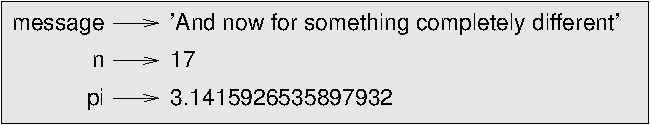
\includegraphics[scale=0.8]{figs/state2.pdf}}
\caption{State diagram.}
\label{fig.state2}
\end{figure}

The type of a variable is the type of the value it refers to.

\begin{verbatim}
>>> type(message)
<type 'str'>
>>> type(n)
<type 'int'>
>>> type(pi)
<type 'float'>
\end{verbatim}



\section{Variable names and keywords}
\index{keyword}

Programmers generally choose names for their variables that
are meaningful---they document what the variable is used for.

Variable names can be arbitrarily long.  They can contain
both letters and numbers, but they have to begin with a letter.
It is legal to use uppercase letters, but it is a good idea
to begin variable names with a lowercase letter (you'll
see why later).

The underscore character, \verb"_", can appear in a name.
It is often used in names with multiple words, such as
\verb"my_name" or \verb"airspeed_of_unladen_swallow".
\index{underscore character}

If you give a variable an illegal name, you get a syntax error:

\begin{verbatim}
>>> 76trombones = 'big parade'
SyntaxError: invalid syntax
>>> more@ = 1000000
SyntaxError: invalid syntax
>>> class = 'Advanced Theoretical Zymurgy'
SyntaxError: invalid syntax
\end{verbatim}
%
\texttt{ 76trombones} is illegal because it does not begin with a letter.
\texttt{ more@} is illegal because it contains an illegal character, \texttt{
@}.  But what's wrong with \texttt{ class}?

It turns out that \texttt{ class} is one of Python's \textbf{ keywords}.  The
interpreter uses keywords to recognize the structure of the program,
and they cannot be used as variable names.
\index{keyword}

Python 2 has 31 keywords:

\begin{verbatim}
and       del       from      not       while
as        elif      global    or        with
assert    else      if        pass      yield
break     except    import    print
class     exec      in        raise
continue  finally   is        return
def       for       lambda    try
\end{verbatim}
%
In Python 3, \texttt{ exec} is no longer a keyword, but \texttt{ nonlocal} is.

You might want to keep this list handy.  If the interpreter complains
about one of your variable names and you don't know why, see if it
is on this list.


\section{Operators and operands}
\index{operator, arithmetic}
\index{arithmetic operator}
\index{operand}
\index{expression}

\textbf{ Operators} are special symbols that represent computations like
addition and multiplication.  The values the operator is applied to
are called \textbf{ operands}.

The operators \texttt{ +}, \texttt{ -}, \texttt{ *}, \texttt{ /} and \texttt{ **}
perform addition, subtraction, multiplication, division and
exponentiation, as in the following examples:

\begin{verbatim}
20+32   hour-1   hour*60+minute   minute/60   5**2   (5+9)*(15-7)
\end{verbatim}
%
In some other languages, \verb"^" is used for exponentiation, but
in Python it is a bitwise operator called XOR.  I won't cover
bitwise operators in this book, but you can read about
them at \url{http://wiki.python.org/moin/BitwiseOperators}.
\index{bitwise operator}
\index{operator!bitwise}

In Python 2, the division operator might not do what you expect:

\begin{verbatim}
>>> minute = 59
>>> minute/60
0
\end{verbatim}
%
The value of \texttt{ minute} is 59, and in conventional arithmetic 59
divided by 60 is 0.98333, not 0.  The reason for the discrepancy is
that Python is performing \textbf{ floor division}.
When both of the operands are integers, the result is also an
integer; floor division chops off the fraction
part, so in this example it rounds down to zero.

In Python 3, the result of this division is a \texttt{ float}.  The new operator
\texttt{ //} performs floor division.
\index{Python 3}
\index{floor division}
\index{floating-point division}
\index{division!floor}
\index{division!floating-point}

If either of the operands is a floating-point number, Python performs
floating-point division, and the result is a \texttt{ float}:

\begin{verbatim}
>>> minute/60.0
0.98333333333333328
\end{verbatim}


\section{Expressions and statements}

An \textbf{ expression} is a combination of values, variables, and operators.
A value all by itself is considered an expression, and so is
a variable, so the following are all legal expressions
(assuming that the variable \texttt{ x} has been assigned a value):
\index{expression}
\index{evaluate}

\begin{verbatim}
17
x
x + 17
\end{verbatim}
%
A \textbf{ statement} is a unit of code that the Python interpreter can
execute.  We have seen two kinds of statement: print and
assignment.

Technically an expression is also a statement, but it is probably
simpler to think of them as different things.  The important difference
is that an expression has a value; a statement does not.


\section{Interactive mode and script mode}

One of the benefits of working with an interpreted language is that
you can test bits of code in interactive mode before you put them
in a script.  But there are differences between interactive mode
and script mode that can be confusing.
\index{interactive mode}
\index{script mode}

For example, if you are using Python as a calculator, you might type

\begin{verbatim}
>>> miles = 26.2
>>> miles * 1.61
42.182
\end{verbatim}

The first line assigns a value to \texttt{ miles}, but it has no visible
effect.  The second line is an expression, so the interpreter
evaluates it and displays the result.  So we learn that a marathon is
about 42 kilometers.

But if you type the same code into a script and run it, you get no
output at all.  In script mode an expression, all by itself, has no
visible effect.  Python actually evaluates the expression, but it doesn't
display the value unless you tell it to:

\begin{verbatim}
miles = 26.2
print miles * 1.61
\end{verbatim}

This behavior can be confusing at first.

A script usually contains a sequence of statements.  If there
is more than one statement, the results appear one at a time
as the statements execute.

For example, the script

\begin{verbatim}
print 1
x = 2
print x
\end{verbatim}
%
produces the output

\begin{verbatim}
1
2
\end{verbatim}
%
The assignment statement produces no output.

\begin{exercise}

Type the following statements in the Python interpreter to see
what they do:

\begin{verbatim}
5
x = 5
x + 1
\end{verbatim}
%
Now put the same statements into a script and run it.  What
is the output?  Modify the script by transforming each
expression into a print statement and then run it again.
\end{exercise}


\section{Order of operations}
\index{order of operations}
\index{rules of precedence}
\index{PEMDAS}

When more than one operator appears in an expression, the order of
evaluation depends on the \textbf{ rules of precedence}.  For
mathematical operators, Python follows mathematical convention.
The acronym \textbf{ PEMDAS} is a useful way to
remember the rules:
\index{parentheses!overriding precedence}

\begin{itemize}

\item \textbf{ P}arentheses have the highest precedence and can be used
to force an expression to evaluate in the order you want. Since
expressions in parentheses are evaluated first, \texttt{ 2 * (3-1)} is 4,
and \texttt{ (1+1)**(5-2)} is 8. You can also use parentheses to make an
expression easier to read, as in \texttt{ (minute * 100) / 60}, even
if it doesn't change the result.

\item \textbf{ E}xponentiation has the next highest precedence, so
\texttt{ 2**1+1} is 3, not 4, and \texttt{ 3*1**3} is 3, not 27.

\item \textbf{ M}ultiplication and \textbf{ D}ivision have the same precedence,
which is higher than \textbf{ A}ddition and \textbf{ S}ubtraction, which also
have the same precedence.  So \texttt{ 2*3-1} is 5, not 4, and
\texttt{ 6+4/2} is 8, not 5.

\item Operators with the same precedence are evaluated from left to
  right (except exponentiation).  So in the expression \texttt{ degrees /
    2 * pi}, the division happens first and the result is multiplied
  by \texttt{ pi}.  To divide by $2 \pi$, you can use parentheses or write
  \texttt{ degrees / 2 / pi}.

\end{itemize}

I don't work very hard to remember rules of precedence for other
operators.  If I can't tell by looking at the expression, I use
parentheses to make it obvious.

\section{String operations}
\index{string!operation}
\index{operator!string}

In general, you can't perform mathematical operations on strings, even
if the strings look like numbers, so the following are illegal:

\begin{verbatim}
'2'-'1'    'eggs'/'easy'    'third'*'a charm'
\end{verbatim}
%
The \texttt{ +} operator works with strings, but it
might not do what you expect: it performs
\textbf{ concatenation}, which means joining the strings by
linking them end-to-end.  For example:
\index{concatenation}

\begin{verbatim}
first = 'throat'
second = 'warbler'
print first + second
\end{verbatim}
%
The output of this program is \texttt{ throatwarbler}.

The \texttt{ *} operator also works on strings; it performs repetition.
For example, \verb"'Spam'*3" is \verb"'SpamSpamSpam'".  If one of the operands
is a string, the other has to be an integer.

This use of \texttt{ +} and \texttt{ *} makes sense by
analogy with addition and multiplication.  Just as \texttt{ 4*3} is
equivalent to \texttt{ 4+4+4}, we expect \verb"'Spam'*3" to be the same as
\verb"'Spam'+'Spam'+'Spam'", and it is.  On the other hand, there is a
significant way in which string concatenation and repetition are
different from integer addition and multiplication.
Can you think of a property that addition has
that string concatenation does not?
\index{commutativity}


\section{Comments}
\index{comment}

As programs get bigger and more complicated, they get more difficult
to read.  Formal languages are dense, and it is often difficult to
look at a piece of code and figure out what it is doing, or why.

For this reason, it is a good idea to add notes to your programs to explain
in natural language what the program is doing.  These notes are called
\textbf{ comments}, and they start with the \verb"#" symbol:

\begin{verbatim}
# compute the percentage of the hour that has elapsed
percentage = (minute * 100) / 60
\end{verbatim}
%
In this case, the comment appears on a line by itself.  You can also put
comments at the end of a line:

\begin{verbatim}
percentage = (minute * 100) / 60     # percentage of an hour
\end{verbatim}
%
Everything from the \texttt{ \#} to the end of the line is ignored---it
has no effect on the program.

Comments are most useful when they document non-obvious features of
the code.  It is reasonable to assume that the reader can figure out
{\em what} the code does; it is much more useful to explain {\em why}.

This comment is redundant with the code and useless:

\begin{verbatim}
v = 5     # assign 5 to v
\end{verbatim}
%
This comment contains useful information that is not in the code:

\begin{verbatim}
v = 5     # velocity in meters/second.
\end{verbatim}
%
Good variable names can reduce the need for comments, but
long names can make complex expressions hard to read, so there is
a tradeoff.


\section{Debugging}
\index{debugging}

At this point the syntax error you are most likely to make is
an illegal variable name, like \texttt{ class} and \texttt{ yield}, which
are keywords, or \verb"odd~job" and \verb"US$", which contain
illegal characters.
\index{syntax error}
\index{error!syntax}

If you put a space in a variable name, Python thinks it is two
operands without an operator:

\begin{verbatim}
>>> bad name = 5
SyntaxError: invalid syntax
\end{verbatim}
%
For syntax errors, the error messages don't help much.
The most common messages are \texttt{ SyntaxError: invalid syntax} and
\texttt{ SyntaxError: invalid token}, neither of which is very informative.
\index{error message}
\index{use before def}
\index{exception}
\index{runtime error}
\index{error!runtime}

The runtime error you are most likely to make is a ``use before
def;'' that is, trying to use a variable before you have assigned
a value.  This can happen if you spell a variable name wrong:

\begin{verbatim}
>>> principal = 327.68
>>> interest = principle * rate
NameError: name 'principle' is not defined
\end{verbatim}
%
Variables names are case sensitive, so \texttt{ LaTeX} is not the
same as \texttt{ latex}.
\index{case-sensitivity, variable names}
\index{semantic error}
\index{error!semantic}

At this point the most likely cause of a semantic error is
the order of operations.  For example, to evaluate
 $\frac{1}{2 \pi}$,
you might be tempted to write

\begin{verbatim}
>>> 1.0 / 2.0 * pi
\end{verbatim}
%
But the division happens first, so you would get $\pi / 2$, which
is not the same thing!  There is no way for Python
to know what you meant to write, so in this case you don't
get an error message; you just get the wrong answer.
\index{order of operations}


\section{Glossary}

\begin{description}

\item[value:]  One of the basic units of data, like a number or string,
that a program manipulates.
\index{value}

\item[type:] A category of values.  The types we have seen so far
are integers (type \texttt{ int}), floating-point numbers (type \texttt{
float}), and strings (type \texttt{ str}).
\index{type}

\item[integer:] A type that represents whole numbers.
\index{integer}

\item[floating-point:] A type that represents numbers with fractional
parts.
\index{floating-point}

\item[string:] A type that represents sequences of characters.
\index{string}

\item[variable:]  A name that refers to a value.
\index{variable}

\item[statement:]  A section of code that represents a command or action.  So
far, the statements we have seen are assignments and print statements.
\index{statement}

\item[assignment:]  A statement that assigns a value to a variable.
\index{assignment}

\item[state diagram:]  A graphical representation of a set of variables and the
values they refer to.
\index{state diagram}

\item[keyword:]  A reserved word that is used by the compiler to parse a
program; you cannot use keywords like \texttt{ if}, \texttt{  def}, and \texttt{ while} as
variable names.
\index{keyword}

\item[operator:]  A special symbol that represents a simple computation like
addition, multiplication, or string concatenation.
\index{operator}

\item[operand:]  One of the values on which an operator operates.
\index{operand}

\item[floor division:] The operation that divides two numbers and chops off
the fraction part.
\index{floor division}

\item[expression:]  A combination of variables, operators, and values that
represents a single result value.
\index{expression}

\item[evaluate:]  To simplify an expression by performing the operations
in order to yield a single value.

\item[rules of precedence:]  The set of rules governing the order in which
expressions involving multiple operators and operands are evaluated.
\index{rules of precedence}
\index{precedence}

\item[concatenate:]  To join two operands end-to-end.
\index{concatenation}

\item[comment:]  Information in a program that is meant for other
programmers (or anyone reading the source code) and has no effect on the
execution of the program.
\index{comment}

\end{description}


\section{Exercises}

\begin{exercise}

Assume that we execute the following assignment statements:

\begin{verbatim}
width = 17
height = 12.0
delimiter = '.'
\end{verbatim}

For each of the following expressions, write the value of the
expression and the type (of the value of the expression).

\begin{enumerate}

\item \texttt{ width/2}

\item \texttt{ width/2.0}

\item \texttt{ height/3}

\item \texttt{ 1 + 2 * 5}

\item \texttt{ delimiter * 5}

\end{enumerate}

Use the Python interpreter to check your answers.
\end{exercise}

\begin{exercise}

Practice using the Python interpreter as a calculator:
\index{calculator}

\begin{enumerate}

\item The volume of a sphere with radius $r$ is $\frac{4}{3} \pi r^3$.
  What is the volume of a sphere with radius 5?  Hint: 392.7 is wrong!

\item Suppose the cover price of a book is \$24.95, but bookstores get a
  40\% discount.  Shipping costs \$3 for the first copy and 75 cents
  for each additional copy.  What is the total wholesale cost for
  60 copies?

\item If I leave my house at 6:52 am and run 1 mile at an easy pace
  (8:15 per mile), then 3 miles at tempo (7:12 per mile) and 1 mile at
  easy pace again, what time do I get home for breakfast?
\index{running pace}

\end{enumerate}
\end{exercise}
